
\section{Access sequences without initial trees: $k$-decomposable permutations}
\label{sec:block_linear}



\subsection{Pattern avoidance and recursive decomposability} 
\label{sec:connection-ext}
We restate and prove Lemma~\ref{lem:connection} that connects  the $k$-decomposability of a permutation with pattern avoidance properties.

\begin{lemma}[Extended form of Lemma~\ref{lem:connection}]
\label{lem:connection-ext}
Let $P$ be a permutation, and let $k$ be an integer. The following statements are equivalent:
\begin{enumerate}[label={{(}\roman*{)}}]
\item $P$ is $k$-decomposable,
\item $P$ avoids all simple permutations of size at least $k+1$,
\item $P$ avoids all simple permutations of size $k+1$ and $k+2$.
\end{enumerate}
\end{lemma}

\begin{proof}
$(ii) \implies (iii)$ is obvious.

$(iii) \implies (ii)$ follows from the result of Schmerl and Trotter~\cite{schmerl_trotter} that every simple permutation of length $n$ contains a simple permutation of length $n-1$ or $n-2$, and the simple observation that if $P$ avoids $Q$, then $P$ also avoids all permutations containing $Q$.

$(ii) \implies (i)$ follows from the observation that a permutation $P$ contains all permutations in its block decomposition tree $\tset_P$. Further, it is known~\cite{brignall} that every permutation $P$ has a block decomposition tree $\tset_P$ in which all nodes are simple permutations. If $P$ contains no simple permutation of size $k+1$ or more, it must have a block decomposition tree in which all nodes are simple permutations of size at most $k$, it is therefore, $k$-decomposable.

$(i) \implies (ii)$: we show the contrapositive $\neg(ii) \implies \neg(i)$. 
Indeed, if $P$ contains a simple permutation $Q$ of size at least $k+1$, then any $k$-decomposition of $P$ would induce a $k$-decomposition of $Q$, contradicting the fact that $Q$ is simple.
\end{proof}


\subsection{$k$-decomposable permutations}
\label{sub:k dec seq}
We prove Lemma~\ref{lem:input-revealing} (v) and (vi). We refer to \S\,\ref{sec:input-rev} for the necessary definitions. We show an example of the gadget $\alt_k$: $$\alt_{7} = \left( \begin{smallmatrix}
  &&&\bullet &&&&\\
  &&&&&\bullet &&\\
  &&\bullet &&&&&\\
  &&&&&&\bullet &\\
  &\bullet &&&&&&\\
  &&&&&&&\bullet \\
  &&&&\bullet &&&\\
 \end{smallmatrix}\right).$$


\begin{lemma}[Lemma~\ref{lem:input-revealing}(v)]
		$\alt_{k+1}$ is a $k$-alternating gadget for \greedy where $\alt_{k}=(\left\lfloor (k+1)/2\right\rfloor,k,1,k-1,2,\dots)$. 
\end{lemma}

\begin{proof}
 

Let $q_{0},\dots,q_{k}$ be
	touch points in $\Greedy(X)$ such that $q_{i}.y<q_{i+1}.y$
	for all $i$ and form $\alt_{k+1}$ with bounding box $B$. 
Suppose that there is no access point in $B$.
	
	
	We prove for $i=1,\dots,k$, that there exists an access point $p_i \in (B.\xmax,n]\times(q_{i-1}.y,q_{i}.y]$ for odd $i$, and $p_i \in [1,B.\xmin)\times(q_{i-1}.y,q_{i}.y]$ for even $i$.

For odd $i$, by \Cref{prop:hidden}~(i), $q_{i}.x$ is hidden in $(q_{i-1}.x,n]$ after $q_{i-1}.y$. So there must be an access point $p_i \in(B.\xmax,n]\times(q_{i-1}.y,q_{i}.y]$, otherwise $q_i$ cannot be touched.  

For even $i$, by \Cref{prop:hidden}~(ii), $q_{i}.x$ is hidden in $[1,q_{i-1}.x)$ after $q_{i-1}.y$. 
	So there must be an access point $p_i \in[1,B.\xmin)\times(q_{i-1}.y,q_{i}.y]$, otherwise $q_i$ cannot be touched.

Observe that $p_{1},\dots,p_{k}$ satisfy $B.\ymin \le p_{1}.y<\dots<p_{k}.y\le B.\ymax$
		and $B.\xmax<p_{i}.x$ for all odd $i$ and $p_{i}.x<B.\xmin$ for all
		even $i$, fulfilling the condition of Definition~\ref{def:gadget}. Hence, $\alt_{k+1}$ is a $k$-alternating gadget.

\end{proof}


\begin{lemma}[Lemma~\ref{lem:input-revealing}(vi)]
	 $\alt_{k+4}$ is a capture gadget for \greedy that runs on $k$-decomposable
		sequence without initial tree.
 
\end{lemma}

\begin{proof}

Let $X$ be a $k$-decomposable permutation.
Since $\alt_{k+4}$ is a $(k+3)$-alternating gadget, if $\alt_{k+4}$ appears in $\Greedy(X)$ with bounding box $B$, then either there is an access point in $B$ or there are access points $p_1, p_2, \dots, p_{k+3}$, satisfying the conditions $B.\ymin \leq p_1.y < \cdots < p_{k+3}.y \leq B.\ymax$ and $B.\xmax < p_i.x$ for odd $i$ and $p_i.x < B.\xmin$ for even $i$. Suppose there is no access point in $B$.


Let $q_0, q_1, \dots, q_{k+3}$ denote the points that form $\alt_{k+4}$ (where $q_0.y < q_1.y < \cdots < q_{k+3}.y$), and let us denote $\pset = \{p_1, \dots, p_{k+3}\}$. Let $\tset$ be a block decomposition tree of $X$ of arity at most $k$. We look at each block $P \in \tset$ as a minimal rectangular region in the plane that contains all access points in the block. 

Let $P^*$ be the \emph{smallest} block in $\tset$ that contains two distinct access points $p_i, p_j \in \pset$ such that $i$ is odd, and $j$ is even. (Observe that $p_i$ is to the right of $B$, and $p_j$ is to the left of $B$.) 

Observe first that the bounding box of $P^*$ must contain or intersect both vertical sides of $B$, otherwise it could not contain points on both sides of $B$. 
Furthermore, the bottom horizontal side of $B$ must be contained entirely in the bounding box of $P^*$: If that were not the case, then there would be no accesses below $B$, and $q_0$ (the lowest point of $\alt_{k+4}$) would not be touched by \greedy (since there is no initial tree).
The following is the key observation of the proof.

\begin{lemma}
\label{lem:d5}
Let $k'$ be the largest integer such that $P^*$ contains $q_0, \dots, q_{k'}$. Then, $k' < k+1$. In words, $P^*$ contains at most the $k+1$ lowest points of $\alt_{k+4}$.
\end{lemma}

\begin{proof}
Let $P^* = \tilde P(P_1,\ldots, P_k)$ be the decomposition of $P^*$ into at most $k$ blocks.
We claim that each block $P_j$ can contain at most one point from $\pset$. First, by the minimality of $P^*$, each block $P_j$ never contains two access points from $\pset$ from different sides of $B$; and $P_j$ cannot contain two points from $\pset$ from the same side of $B$ either, because assuming otherwise that $P_j$ contains two points from $\pset$ from the left of $B$, it would follow that there is another access point $(a,t) \in \pset$ on the right of $B$ outside of $P_j$ such that $(P_j).\ymin < t< (P_j).\ymax$, contradicting that $P_j$ is a block.  

Observe further that, except for the block containing $p_1$, each block $P_j$ cannot overlap with $B$. %% (we remark that the block $P_j$ that contains $p_1$ can overlap with the corner of $B$.)   
Since we have at most $k$ such blocks in the decomposition, and because $q_i.y \ge p_i.y$ for all $i$, it follows that the top boundary of $P^*$ must be below $q_{k+1}$.  
 
\end{proof}

Since the bounding box of $P^*$ contains (at best) the first $k+1$ points of $\alt_{k+4}$, the three remaining points of $\alt_{k+4}$ need to be touched after the last access in $P^*$. In the following we show that this is impossible.

Let $(L, t_L)$ be the topmost access point inside $P^*$ to the left of $B$, such that there is a touch point inside $B$ at time $t_L$. Let $(R, t_R)$ be the topmost access point inside $P^*$ to the right of $B$, such that there is a touch point inside $B$ at time $t_R$. Let $L'$ be the rightmost element inside $B$ touched at time $t_L$, and let $R'$ be the leftmost element inside $B$ touched at time of $t_R$.

\begin{lemma}
\label{lem:onlybetween}
After time $t_L$, within the interval $[B.\xmin, L']$, only $L'$ can be touched. Similarly, after time $t_R$, within the interval $[R', B.\xmax]$, only $R'$ can be touched. 
\end{lemma}

\begin{proof}
Let $L''$ be the rightmost touched element in $[L,B.\xmin)$ at time $t_L$, and let $R''$ be the leftmost touched element in $(B.\xmax, R]$ at time $t_R$. 

%, and no access to an element in $(B.\xmax, R'')$,
%$Let $t^* = (P^*).\ymax$. 
We have that $\tau(L'',t_L), \tau(L',t_L) \geq \tau(x,t_L)$, for any $x \in [B.\xmin, L')$. Thus, any $x \in [B.\xmin, L')$ is hidden in $(L'',L')$ after $t_L$.

Above $P^*$ there can be no access to an element in $[L'',L']$, since that would contradict the fact that $P^*$ is a block. Within $P^*$ after $t_L$ there can be no access to an element in $(L'',B.\xmin)$, as the first such access would necessarily cause the touching of a point inside $B$, a contradiction to the choice of $(L,t_L)$. An access within $B$ is ruled out by our initial assumption.

Thus, there is no access in $(L'',L') \times (t_L,n]$, and from Lemma~\ref{prop:hidden}(iii) it follows that any $x \in [B.\xmin, L')$ can not be touched after time $t_L$.

We argue similarly on the right side of $B$.
\end{proof}

As a corollary of Lemma~\ref{lem:onlybetween}, note that above $P^*$ only elements within $[L',R']$ can be touched within $B$. %%We will argue that at most two different elements of this interval are touched outside of $P^*$. 
If $L' = R'$, then only one element can be touched, and we are done. Therefore, we assume that $L'$ is strictly to the left of $R'$.


We assume w.l.o.g.\ that $t_R > t_L$ (the other case is symmetric). Let $(Q,t_Q)$ be the first access point left of $B$ with $t_Q > t_R$ such that there is a touch point inside $B$ at time $t_Q$. Observe that $(Q,t_Q)$ is outside of $P^*$ by our choice of $(L,t_L)$. If no such $Q$ exists, we are done, since we contradict the fact that $\alt_{k+4}$ is a $(k+3)$-alternating gadget. 

Let $(Z, t_Z)$ denote the last touch point with the property that $Z \in [(P^*).xmin, L')$, and $t_Z \in [t_L, t_Q)$. If there are more such points in the same row, pick $Z$ to be the leftmost. Note that $(Z, t_Z)$ might coincide with $(L, t_L)$. We have $t_Z \le t_R$ because otherwise $(Q,t_Q)$ cannot exist. Note than $t_Z > t_R$ would imply that elements in $[L',R']$ are hidden in $(Z,R)$ after $t_R$. 

Next, we make some easy observations.

\begin{lemma}
\label{lem:emptiness}
The following ranges are empty:
\begin{enumerate}[label={{(}\roman*{)}}]
\item $[B.\xmin, B.\xmax] \times [t_R+1, t_Q-1]$,
\item $[1, Z-1] \times [t_Z+1, t_R]$,
\item $[Q, Z-1] \times [t_Z+1, t_Q-1]$,
\item $[Q, R'-1] \times [t_{R}+1, t_Q-1]$.
\end{enumerate}
\end{lemma} 

\begin{proof}

\begin{enumerate}[label={{(}\roman*{)}}]
\item It is clear that there can be no access point inside $B$ by assumption. Suppose there is a touch point in $[B.\xmin, B.\xmax] \times [t_R+1, t_Q-1]$, and let $(Q',t_{Q'})$ be the first (lowest) such point. Denote the access point at time $t_{Q'}$ as $(Q'', t_{Q'})$. Clearly $t_{Q'}>(P^*).\ymax$ must hold, otherwise the choice of $(L,t_L)$ or $(R,t_R)$ would be contradicted. Also $Q''>(P^*).\xmax$ must hold, otherwise the choice of $(Q,t_Q)$ would be contradicted.

But this is impossible, since $Q' \in [L',R']$, and $\tau(Q',t_{Q'}-1) \leq t_R$, and thus the rectangle with corners $(Q'', t_{Q'})$ and $(Q', \tau(Q',t_{Q'}-1))$ contains the touch point $(R,t_R)$, contradicting the claim that \greedy touches $Q'$ at time $t_{Q'}$. 
\item 
All elements in $[1, Z-1]$ are hidden in $[1,Z-1]$ after $t_Z$. There can be no access points on the left of $P^*$, due to the structure of the block decomposition, and there is no access point in $[(P^*).\xmin, Z-1] \times [t_Z+1, t_Q-1]$ due to the choice of $Z$.  
%No touched points because of hiding arguments and the choice of $Z$.
%Moreover, during the time $[t_Z+1, t_R]$, all accesses are on the right of $Z$ (again from the choice of $(Z,t_Z)$), and 
Hence there cannot be a touch points in $[1,Z-1] \times [t_Z+1, t_R]$.  
\item First there is no access point in $[Q,Z-1] \times [t_Z+1,(P^*).\ymax]$ due to the choice of $(Z,t_Z)$ and the structure of block decomposition. 
Also, there is no access point in $[Q,Z-1] \times ((P^*).\ymax, t_Q-1]$: Assume there were such an access point $(Q',t_{Q'})$. Then it must be the case that $Q < Q' < (P^*).\xmin$ and $(P^*).\ymax < t_{Q'} < t_Q$. 
Any rectangle formed by $(Q,t_Q)$  and a point in $P^* \cap B$ would have contained $(Q',t_{Q'})$, a contradiction to the fact that \greedy touches a point inside $B$ at time $t_Q$. 

Next, we argue that there is no non-access touch point $(a,t) \in [Q,Z-1] \times [t_Z+1,t_Q-1]$. 
There are three cases.  
\begin{compactenum}[--]
\item $(a,t) \in [(P^*).\xmin, Z-1] \times [t_Z+1,t_Q-1]$ contradicts the choice of $(Z,t_Z)$.

\item $(a,t) \in [Q,(P^*).\xmin) \times [t_Z+1, (P^*).\ymax]$ contradicts the fact that all elements in $[1,Z)$ are hidden in $[1,Z)$ after $t_Z$, and there is no access in $[1,Z)$ in the time interval $[t_Z+1,(P^*).\ymax]$, since $P^*$ is a block. 
%% if $a>(P^*).\xmin$, we contradict the choice of $(Z,t_Z)$. 
%%If $a < (P^*).\xmin$, we know that $a$ is $[t_Z+1, \mtop(P^*)]$-hidden via $[0,Z-1]$.  
\item $(a,t) \in [Q,(P^*).\xmin) \times ((P^*).\ymax,t_Q-1]$, contradicts the claim that at time $t_Q$ \greedy touches a point inside $B$, since any rectangle formed by $(Q,t_Q)$  and a point in $P^* \cap B$ would have contained $(a,t)$.
\end{compactenum} 
 
%Hiding arguments and the choice of $Q$.
\item
Given the previous claims, it remains only to prove that there is no touch point $(a,t) \in [Z, B.\xmin) \times t \in [t_R+1, t_Q-1]$.
There cannot be such a touch point for $t \leq (P^*).\ymax$ due to the choice of $(Z,t_Z)$. For $t > (P^*).\ymax$, there cannot be souch an access point due to the structure of block decomposition. Remains the case when $(a,t)$ is a non-access touch point in $[Z,B.\xmin) \times ((P^*).\ymax, t_Q-1$. This is also impossible, as any rectangle formed by $(Q,t_Q)$ and a point in $P^* \cap B$ would have contained $(a,t)$, contradicting the choice of $(Q,t_Q)$. 

%Hiding arguments and the choice of $R$, $R'$, $Q$.
\end{enumerate} 
\end{proof}


\begin{lemma}
\label{lem:d8}
At time $t_Q$ %if we touch an element in $[L',R']$, then 
we touch $R'$. Let $L^*$ be the leftmost element touched in $[L',R']$ at time $t_Q$ (it is possible that $L^* = R'$). After time $t_Q$, only $L^*$ and $R'$ can be touched within $[L',R']$. 
%%%, because $[L',L'')$ is blocked by $X$. If $L''$ does not exist, it means that $X$ blocks $[L',R')$, so only $R'$ can be touched.
\end{lemma}
\begin{proof}
The first part follows from the emptiness of rectangles in Lemma~\ref{lem:emptiness}.
That is, the lemma implies that the rectangle formed by $(Q,t_Q)$ and $(R', t_R)$ is empty, so \greedy touches $R'$ at time $t_Q$.  

%The second part follows from hiding arguments.
The elements $a \in (L^*, R')$ cannot be touched because they are hidden in $(L^*,R')$ after $t_Q$, and there is no access point in this range after $t_Q$, due to the structure of the block decomposition.
Suppose that some element $a \in [L', L^*)$ is touched (for the first time) at some time $t > t_Q$ by accessing element $x$. 
So the rectangle formed by $(x,t)$ and $(a,\tau(a,t-1))$ is empty, and we know that $\tau(a,t-1) < t_R$. Notice that $x<(P^*).\xmin$ for otherwise $(R,t_R)$ would have been in the rectangle formed by $(x,t)$ and $(a,\tau(a,t-1))$, a contradiction.
Furthermore, $\tau(a,t-1) > t_Z$ for otherwise, $(Z,t_Z)$ would have been in the rectangle formed by $(x,t)$ and $(a,\tau(a,t-1))$, a contradiction. 
Now, since $\tau(a,t-1) > t_Z$, Lemma~\ref{lem:emptiness} implies that the rectangle formed by $(Q,t_Q)$ and $(a,\tau(a,t-1))$ must be empty, therefore $a$ is touched at time $t_Q$; this contradicts the choice of $L^*$. 

\end{proof}

Lemma~\ref{lem:d5}, \ref{lem:onlybetween}, and \ref{lem:d8} together imply that in total at best the $k+3$ lowest points of $\alt_{k+4}$ can be touched (out of the $k+4$ needed). This means that our assumption that $B$ is free of access points was false. Therefore $\alt_{k+4}$ is a capture gadget, finishing the proof of Lemma~\ref{lem:input-revealing}(vi). See Figure~\ref{proof_slide} for an illustration.

\begin{figure}
\begin{center}  
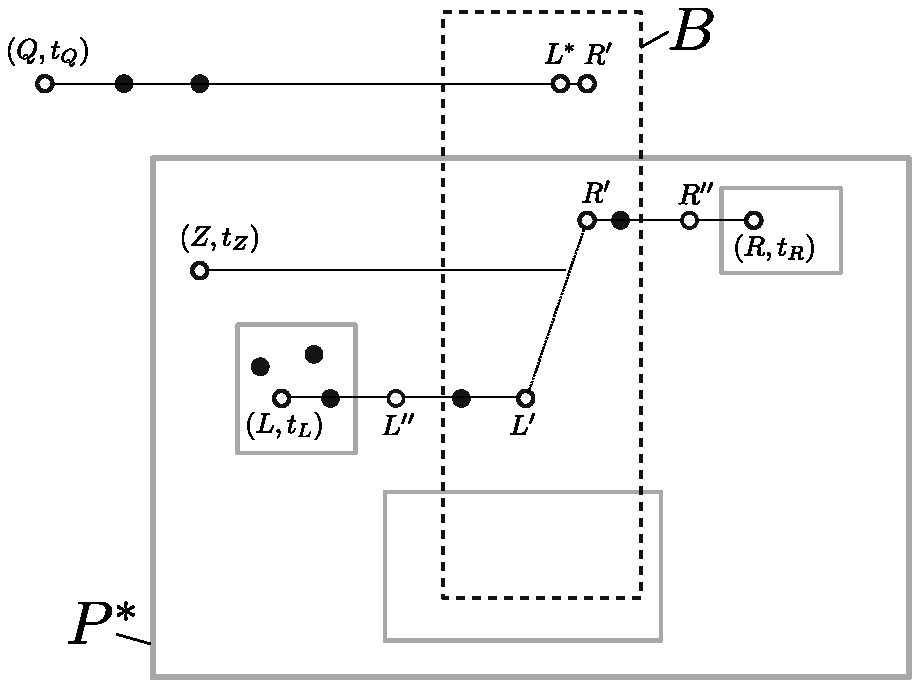
\includegraphics[scale=0.7]{block_fig.pdf}
\end{center}
\caption{Illustration of the proof of Lemma~\ref{lem:input-revealing}(vi).} 
\label{proof_slide}
\end{figure}
\end{proof}

\iffalse
\subsection{Alternative direct proof for preorder sequences}
\label{sec:alt-direct}

We give an alternative proof of Theorem~\ref{thm:greedy-traversal}.

\begin{lemma}(F\"{u}redi, Hajnal~\cite[Cor.\ 2.7]{furedi_hajnal})~~ Let $M$ be an $n \times m$ matrix. If $M$ is $(231)$-free, then $w(M) \leq 2(m+n)$.
\end{Lemma}

Recall that a preorder sequence is $231$-free, and observe that $(231) = \alt_3$. Let $X \in {\sf PreOrd}_n$. We use Lemma~\ref{lem:input-revealing} (v).
\fi

